\section{Introduction}
The Control Panel (CP) is a Django web application which offers a unified interface to configure and manage the platform. Its graphical interface gives to the editors a menu with options to access the different modules available on the system. It offers a unified interface to configure and administrate the platform. For example, the Editors can remove unused experiments for the archive or add new images to a demo.

Thr CP provides a navigation menu panel for each module. For example, one of the panels is Status, which shows a list of the modules with summarized information about them, allowing the user to monitor if they are currently running. Another panel is the Archive Module, which provides a list of the demos with stored experiments, as a result of an execution with original data. It allows the editor to remove specific experiments upon request (e.g., inappropriate images). There is also a Blobs Module option, which allows to add and remove blobs for a particular demo. The DemoInfo panel permits the user to access information about the demos, authors and editors stored on the IPOL demo system, organized in three sections.
%
The Demos section is the option selected by default, and makes it possible to edit the demo metadata, such as its ID, title, or the source code URL, the assigned editors, or its support scripts, among others. Fig. \ref{fig:control_panel} shows a screen capture of the Control Panel application as shown in the browser.

\begin{figure}[!ht]
    \centering
    \tcbox[sharp corners, boxsep=0.0mm, boxrule=0.1mm, colback=white]{
        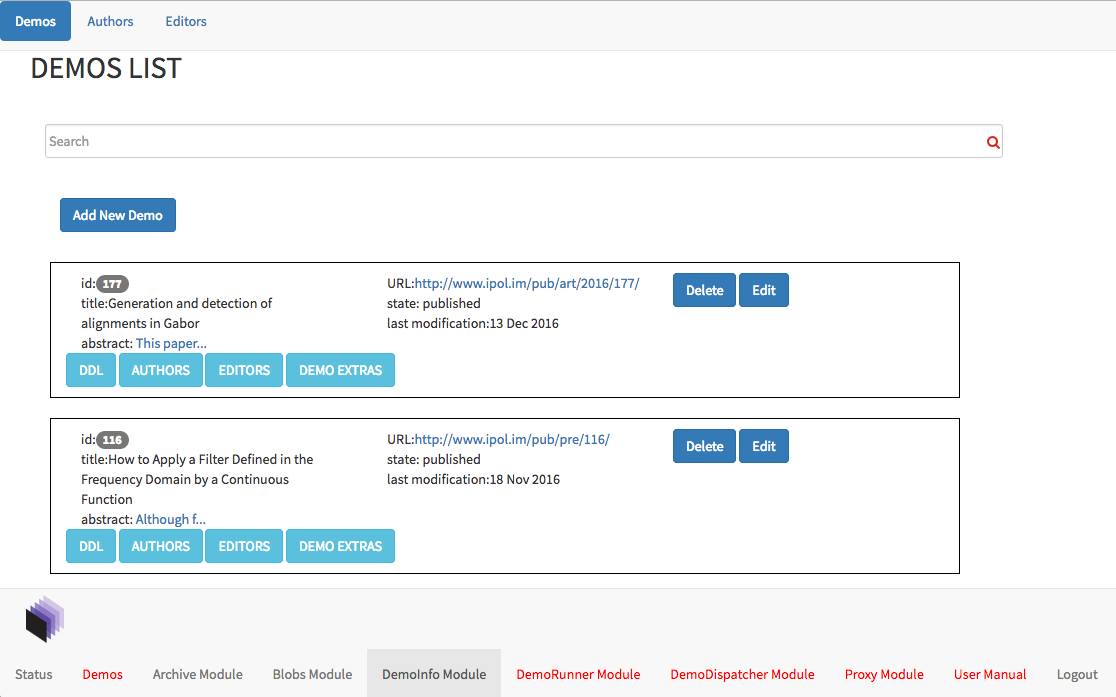
\includegraphics[width=0.8\columnwidth]{images/cp.png}
    }
    \caption{List of demos in the DemoInfo panel.}
    \label{fig:control_panel}
\end{figure}
